\chapter{Referencial Teórico}
Este capítulo apresenta os conceitos de entropia, métricas socias, métricas de autoria e métricas de processo.

\section{Entropia de mudança}
A entropia de \citeonline{Shannon:2001:MTC:584091.584093} é uma medida para mensurar a incerteza associada a uma variável que quantifica uma informação contida em uma mensagem produzida por um emissor de dados. A partir dessa definição foi criado o conceito de entropia de mudança que tem como objetivo indicar o quanto um código está mudando durante um determinado período de tempo. 

Na entropia de mudança o software é considerado o emissor de dados e as modificações realizadas são os dados de entrada. A entropia é uma medida para mensurar a quantidade de mudanças que ocorreram em um determinado espaço de tempo em um arquivo de um projeto. As mudanças consideradas podem ser obtidas a partir da quantidade de linhas modificadas em um intervalo de tempo ou utilizando número de \textit{commits}.

A entropia de mudança é definida como \cite{Hassan:2009:PFU:1555001.1555024}:

\begin{equation}
H(S) = {\sum\limits_{n=1} }\frac{chg(f_i)}{chg(S)}log_2(\frac{chg(f_i)}{chg(S)})
\end{equation}

A figura 2.1 mostra um exemplo do cálculo da entropia dos arquivos de um sistema \cite{Hassan:2009:PFU:1555001.1555024}. Nesse exemplo é considerado os arquivos A, B, C e D de um sistema dado um período de tempo qualquer, na qual as estrelas indicam quando ocorreu uma mudança no arquivo.

\begin{figure}[h]
	\captionsetup{justification=centering}
	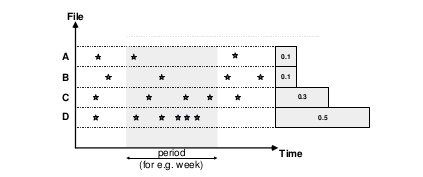
\includegraphics[width=\linewidth]{entropiamudanca.png}
	\caption{Exemplo de cálculo de entropia de mudança por arquivo \cite{Hassan:2009:PFU:1555001.1555024}.}
	\label{figura:entropiaimagem}
\end{figure}

Para cada arquivo no sistema, é feito a contagem de quantas vezes ele foi modificado em um período e depois é dividido pelo total de mudanças que ocorreram nesse mesmo período considerando todos os arquivos. Por exemplo, na figura 2.1 como ocorreram dez mudanças no período selecionado e uma mudança no arquivo A nesse mesmo paríodo então a entropia de mudança para esse arquivo é 0,1.

\subsection{Trabalhos Relacionados}
No trabalho de \citeonline{Hassan:2009:PFU:1555001.1555024} foi introduzido o conceito de entropia de mudança do software e foi feito um modelo básico de mudança de código (BCC - \textit{Basic Code Change Model}) para mensurar a complexidade de mudança.

No modelo básico de mudança de código são utilizados arquivos como unidade de código para mensurar a complexidade de código, o intervalo de tempo para o cálculo da entropia é fixo e é considerado que os arquivos do projeto sejam sempre os mesmos. Para eliminar a limitação do tempo e a limitação alteração no número arquivos é utilizado o modelo extendido de mudança de código (ECC).

No ECC o histórico de mudanças é dividido em períodos de tamanhos iguais. Essa divisão pode ser feita com base em diferentes critérios: com base no tempo, no número de modificações ou em períodos onde ocorrem mais modificações (\textit{Burst Based Period}). A entropia será calculada com base no número de modificações que ocorreram no período definido.

\citeonline{Hassan:2009:PFU:1555001.1555024} aplicou o modelo ECC para 6 projetos: NetBSD, FreeBSD, OpenBSD, Postgres, KDE e KOffice. Nesse estudo foi comparado modelos de predição de defeitos baseados na entropia, modelo baseados em defeitos anteriores e modelo baseado em modificações anteriores.

Os resultados indicam que modelos baseados na métrica de entropia tem o desempenho igual ou superior aos modelos baseados em modificações anteriores e baseados em defeitos anteriores.

A pesquisa de \citeonline{Canfora2014} relaciona a entropia de mudança com características do software e atividades de desenvolvimento. As características analisadas foram: refatoração, número de commiters, padrões de projetos e nome de tópicos no projeto. Na pesquisa foram analisados os projetos ArgoUML, Eclipse-JDT, Mozilla e Samba em um período de cerca de 10 anos.

O método para extração de dados foi dividido em 6 passos: extração das métricas de mudança do sistema de controle de versão, cálculo da entropia de mudança, identificação das mudanças relacionadas a refatoração, contagem número de autores que contribuem para o projeto, identificação dos padrões de projetos e por último foi necessário identificar os tópicos que são descritos na mensagem de cada \textit{commit}. 

Os resultados de Canfora indicam que a entropia de mudança diminui de forma significante após uma atividade de refatoração, o valor da entropia é mais alto para arquivos com maior número de contribuidores, classes que participam de diferentes padrões de projetos exibem valores diferentes de entropia, mudanças classificadas em diferentes tópicos exibem valores de entropia diferentes e há maior relação entre o valor da entropia, tópicos de mudança e número de desenvolvedores que modificam um arquivo. 

\section{Métricas}
Métricas de software são medidas para mensurar características presentes no desenvolvimento de software e servem para auxiliar na tomada de decisões durante o desenvolvimento do projeto \cite{koscianski2007qualidade}. As métricas foram divididas em métricas de autoria, sociais e de processo. 

As métricas de autoria medem a contribuição do desenvolvedor nos projetos, métricas sociais medem a interação entre os desenvolvedores e as métricas de processo mensuram as mudanças que ocorreram em relação aos artefatos criados durante o desenvolvimento do projeto.

\subsection{Métricas de autoria}
Esta seção apresenta métricas calculadas a partir das contribuições dos usuários em cada arquivo de um projeto.

\subsubsection{\textit{Authorship}}
Authorship é uma medida para mensurar o quanto um desenvolvedor contribuiu para um determinado módulo de software.

Essa medida pode ser obtida de várias formas: contando número de arquivos que o desenvolvedor modificou, número de commits e outra possibilidade é contar número de linhas modificadas pelo contribuidor, também chamada de code churn\cite{Munson:1998:CCM:850947.853326}.

Na pesquisa realizada por \citeonline{Rahman2011} o authorship é calculado utilizando o número de linhas modificadas no código pelo desenvolvedor dividido pelo número total de linhas do arquivo, e o autor com a maior contribuição é denomidado ownership. Também é definido implicated code, que é o código modificado quando é corrigido um determinado erro no módulo de software. O trabalho de Rahman investiga a relação entre ownership, authorship e experience com implicated code. Para cada linha de código modificado é utilizado o comando blame para identificar o autor responsável por essa mudança. O resultado fornece evidências indicando que implicated code tende a ser mais frequentemente gerado por poucos autores, vários fragmentos de códigos modificados tem apenas um único autor.

\subsubsection{\textit{Ownership}}
No trabalho de \citeonline{Greiler} o Ownership é medido considerando número de contribuidores de um arquivo e também é verificado se existe um contribuidor principal, nesse caso a medida foi calculada com base no número de commits do autor em relação ao total de commits para aquele componente.

No artigo de \citeonline{Foucault2015} os contribuidores são classificados como owner, minor e major. Owner é o contribuidor com maior valor de contribuição, minor o desenvolvedor que contribuiu com menos de 5\% e major contribuiu com mais de 5\%.

A métrica social ownership será usada para se referir ao authorship do desenvolvedor que mais contribuiu com o projeto \cite{Thongtanunam}. 

\subsubsection{Experiência}
A experiência é a medida para calcular o nível de experiência do contribuidor, essa medida é computada analisando o número de linhas \cite{Rahman2011} deltas comitadas pelo contribuidor em determinado espaço de tempo.

Na pesquisa de \citeonline{Rahman2011} a experiencia é dividida em dois tipos: a experience especializada e experience geral. A experience especializada é medida considerando o quanto um indivíduo contribui em um determinado arquivo e a experiência geral é medida conseiderando um projeto inteiro.

\subsection{Métricas Sociais}
Esta seção apresenta métricas calculadas a partir da comunicação entre os desenvolvedores a partir das issues e de Pull Requests. As métricas são descritas na tabela 2.1.

\begin{table}[]
\centering
\caption{Tabela de métricas sociais}
\label{metricasociais}
\begin{tabular}{|p{3cm}|p{12cm}|}
\hline
Métrica                                          & Descrição                                                                                                                              \\ \hline
Pull Requests fechados por arquivo               & Representa o número total de Pull Request fechados onde determinado arquivo do projeto foi modificado.                                 \\ \hline
Pull Request abertos por arquivo                 & Representa o número total de Pull Requests abertos onde determinado arquivo do projeto foi modificado.                                 \\ \hline
Comentários em Pull Request abertos  & Representa o número total de comentários considerando todos os Pull Request abertos até o momento para determinado arquivo do projeto  \\ \hline
Comentários em Pull Request fechados & Representa o número total de comentários considerando todos os Pull Request fechados até o momento para determinado arquivo do projeto \\ \hline
\end{tabular}
\end{table}

\subsection{Métricas de processo}
As métricas de processo são métricas para mensurar as características relacionadas aos artefatos produzidos durante o desenvolvimento do projeto. As métricas de processo serão descrita na tabela 2.1 e serão calculadas utilizando a ferramenta Change Metrics:

\begin{table}[]
\centering
\caption{Tabela de métricas de processo}
\label{my-label}
\begin{tabular}{|p{3cm}|p{12cm}|}
\hline
Nome da métrica                  & Descrição                                                                                                                                                                         \\ \hline
Quantidade de commits            & A quantidade de commits representa o nível de atividade do projeto em termos de número de commits feitos. È calculado o número de commits do projeto em um certo perído de tempo. \\ \hline
Quantidade de defeitos           & A quantidade de defeitos será calculado com o número de issues do projeto que foram criadas em uma determinada data.                                                              \\ \hline
Idade do arquivo             & A métrica idade do arquivo representa o tempo de existência do arquivo. O cálculo é utilizado medindo a diferença de tempo entre o primeiro e último commit.                  \\ \hline
Quantidade de linhas removidas   & Essa medida representa a quantidade de linhas removidas de um arquivo até o momento.                                                                                              \\ \hline
Quantidade de linhas adicionadas & Essa medida representa a quantidade de linhas adicionadas de um arquivo até o momento.                                                                                            \\ \hline
Code Churn                       & A métrica Code Churn representa a soma de todas as linhas de código removidas e adicionas no arquivo.                                                                             \\ \hline
Quantidade de refatorações       & Essa medida representa a quantidade de refatorações ocorridas até o momento, se a refatoração é citada no commit.                                                                 \\ \hline
Max Change Set                   & A métrica Max Change Set representa o número máximo de arquivos que foram alterados junto com o arquivo em questão.                                                               \\ \hline
Average Change Set               & As métricas Average Change Set representa a média de número de arquivos alterados juntos.                                                                                         \\ \hline
\end{tabular}
\end{table}
